\section{Aims}
% general intro
Here I describe COATi (COdon-aware Alignment Transducer), a new statistical
aligner that can handle artifacts in genomic datasets and employs robust models
of molecular evolution.
% \green{This aligner will be capable of handling all types of alignment problems,
% including non-coding DNA, with a prime focus on modeling coding sequences.}

\subsection{Aim 1 - Statistical Pairwise Alignment of Protein Coding Sequences}
% Talk about pairwise alignment

% pair-HMM vs FSTs.
\subsubsection{Pairwise hidden Markov models.}
Statistical alignment is typically performed using pairwise hidden Markov
models (pair-HMMs).
Pair-HMMs are computational machines with two output tapes and a set of states
that emit symbols onto one or both tapes.
A path through a pair-HMM represents a possible alignment between the two
sequences.
Conceptually, these machines generate two sequences (X and Y) from an unknown
common ancestor and calculate the probability that two sequences are related,
represented $P(X,Y)$ \parencite{yoon_2009_hmm}.
Pair-HMMs have the ability to rigorously model molecular sequence evolution and
can find an optimal alignment, among other capabilities.
% (Forward algorithm), estimate optimal alignment (Viterbi),
% and estimate model parameters (Baum-Welch).

\subsubsection{Finite state transducers (FSTs)}

\begin{wrapfigure}[16]{r}{0.35\textwidth}
\vspace{-2em}
\centering
\begin{framed}
    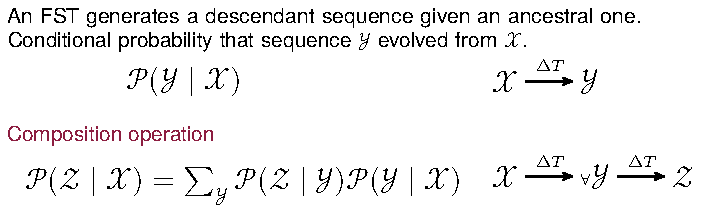
\includegraphics[scale=1]{fig-fst.pdf}
    \caption{(a) Pair-HMMs can generate the probability that two sequences are
             related. (b) FSTs can generate the probability that sequence $Y$
             evolved from sequence $X$.}
    \label{fig:fst}
\end{framed}
\end{wrapfigure}

A limitation of pair-HMM is the ability to only model evolution of two related
sequences from an unknown ancestor, thus not being able to use the output of one
pair-HMM as the input of another.
Finite-state transducers (FSTs) share similar computational characteristics as
pair-HMMs and have an input and output tape, instead of two output tapes.
FSTs absorb symbols from an input tape and emit symbols to an output tape.
Conceptually, an FST generates a descendant sequence given an ancestral one
$X \Rightarrow Y$.
Properly weighted, an FST can calculate the conditional probability that
sequence $Y$ evolved from sequence $X$, represented $P(Y|X)$.

FSTs have similar benefits to pair-HMMs in addition to well established
algorithms for combining them in different ways
\parencite{bradley2007transducers}.
A powerful and versatile algorithm is composition, which consists of sending the
output of one FST as the input of a second one.
% This allows $P(Z|X) = \sum_Y P(Z|Y) P(Y|X)$, represented $X \Rightarrow$
% $Y$ $\Rightarrow Z$.
In the development of COATi I will design complex FSTs from smaller FSTs, each
representing a specific process.

\subsubsection{Evolution FST}

% evolution fst intro
The evolution FST is based on existing transducers
(e.g. \cite{holmes2001evolutionary}).
This FST is formed by composing a substitution FST (Fig.
\ref{fig:evolution-fst}-a) that models codon evolution and an indel FST (Fig.
\ref{fig:evolution-fst}-b) that models insertions and deletions, including
frameshifts.
The power of this FST with respect to others is the combination of a codon
substitution model with gaps that can occur at any position in any length.

\begin{figure}[h!]
\begin{framed}
\centering
    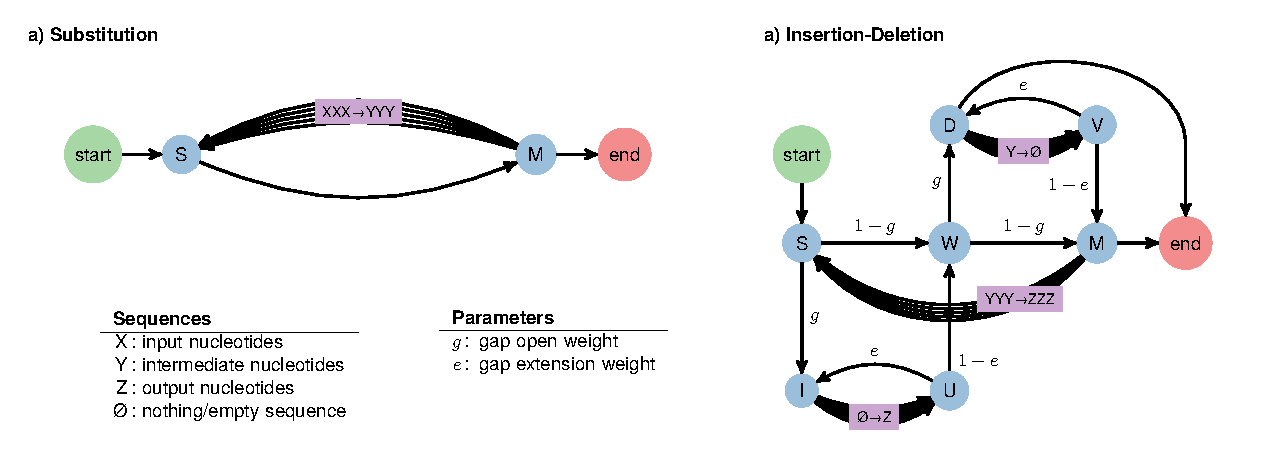
\includegraphics[width=\textwidth]{fig-evolution-fst.pdf}
    \caption{The evolution FST is assembled by composing a substitution FST and
    an indel FST. Each node represents a state in an FST while arcs display
    possible transitions between states (and their weights). Absorption and
    emission of symbols occurs between states. (a) The substitution FST
    encodes a 64x64 codon substitution model with 64 arcs from M to S. (b)
    The indel FST allows for insertions (I to U) and deletions (D to V).
    Contiguous insertions and deletions are always arranged for insertions to
    precede deletions to limit equivalent alignments.}
    \label{fig:evolution-fst}
\end{framed}
\end{figure}

% \vspace{2em}

\textbf{Substitution model.}
% substitution model
Codon substitution models are uncommon in sequence aligners, despite their
extensive use in phylogenetics.
COATi will support an abundance of codon models by using a continuous-time
Markov model, with instantaneous substitution rate matrix $Q$:\\
%  Q matrix
\begin{align*} Q_{ij} &= \begin{cases}
    \mu_{ij} & \text{if $i$ and $j$ are synonymous}\\
    \omega \cdot \mu_{ij} & \text{if $i$ and $j$ are nonsynonymous}
    \end{cases}\\[10pt]
   Q_{ii} &= -\sum_{j:j \neq i} Q_{ij}
\end{align*}

where each position in $Q$ defines the rate that codon $i$ changes to codon $j$
and total rate for each row is zero.
Model parameter $\mu_{ij}$ is the mutation rate of codon $i$ to $j$ and $\omega$
represents the strength of selection for amino acid changes.
The substitution probability after time $t$ is calculated via matrix
exponentiation $P(j|i;t) = e^{Qt}$.

\begin{wrapfigure}[15]{r}{0.5\textwidth}
    \vspace{-1.5em}
    \centering
    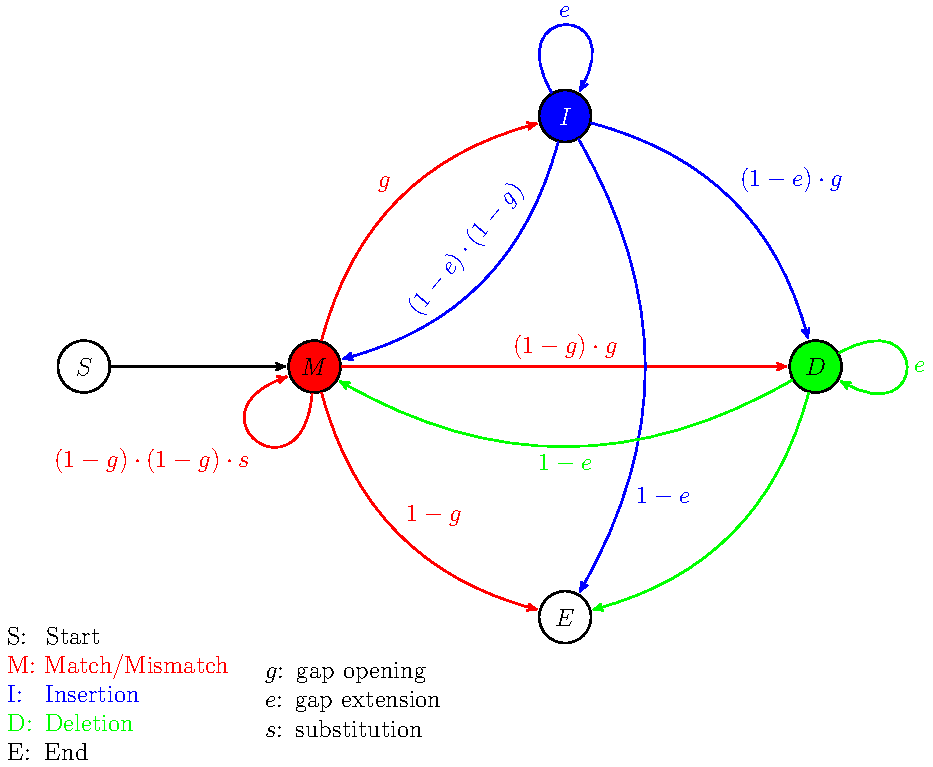
\includegraphics[scale=0.6]{fig-dp-model.pdf}
    \caption{Simplified evolution FST, maintaining the exact transition weights.}
    \label{fig:dp-model}
\end{wrapfigure}

% different ways to select parameter values
COATi will offer different ways to specify mutation rates ($\mu$), including
built-in models such as Muse and Gaut (MG94) \parencite{muse_gaut_1994},
empirical codon model (ECM) \parencite{kosiol_ECM_2007}, and the ability to read
user-provided models via an input file.

% summary paragraph
% \textbf{COATi alignpair.}
% COATi will be a powerful statistical pairwise aligner that benefits from
% robust and modern codon substitution models that allows gaps at any position and
% offers the ability to control model parameters such as substitution rates,
% selection, and indel distributions.
% Coati-alignpair will be capable of finding the optimal alignment between two
% sequences (Viterbi
% algorithm) and the probability that the sequences are related (Forward algorithm).

\subsubsection{Dynamic programming}

Composition is one of the most powerful operations on FSTs, as it allows complex
FSTs to be build from smaller and simpler parts.
However, composing many large FSTs is expensive and can be prohibitive.
Despite the existence of efficient C++ FST libraries, runtime is still limiting
when dealing with sequences longer than a few thousand nucleotides.

To solve this issue, the search for an optimal path (alignment) through the
evolution FST can be reformulated as a dynamic programming problem.
Maintaining the statistical framework, COATi will implement a Gotoh-inspired
algorithm thus reducing the problem to a manageable $\mathcal{O}(nm)$
runtime, where $n$ and $m$ are the length of the sequences.
This can be further improved via Myers and Miller \parencite{myers_miller_1988},
which implements a divide and conquer approach.

% \subsubsection{Validation}
% \textbf{Simulated data.}
% simulated data is an almost mandatory step in every tool validation process
% this will be done by simulating alignments with different values for substitution
%  and indel rates as well as divergence (?)
% To make this step more realistic, gap patterns will be inferred from real data
%  alignments.
% \textbf{Real/biological data.}
% \begin{itemize}
%     \item maybe comment that all current alignment benchmarks are AA?
%     \item probably use some "downstream analysis" result for validation (comparison)
% \end{itemize}
